\chapter{Лекция 4. Метрические характеристики графа. Способы представления. Связность}

% === Метрические характеристики ===

$G(V, E)$ --- неориентированный, связный граф.

\begin{defn}{Расстояние между вершинами}{distance}
$\forall\, u, v \in V$:
\[
  \operatorname{dist}(u, v) := \min l,
\]
где $l$ --- длина пути $u \to \ldots \to v$.

Свойства:
\begin{itemize}
  \item $\operatorname{dist}(u, u) = 0$;
  \item $\operatorname{dist}(u, v) = \operatorname{dist}(v, u)$.
\end{itemize}
\end{defn}

\begin{defn}{Эксцентриситет вершины}{eccentricity}
$v \in V$:
\[
  \varepsilon(v) := \max_{u \in V} \bigl\{\operatorname{dist}(u, v)\bigr\}.
\]
\end{defn}

\begin{defn}{Радиус графа}{radius}
\[
  R(G) := \min_{v \in V} \bigl\{\varepsilon(v)\bigr\}.
\]
\end{defn}

\begin{defn}{Диаметр графа}{diameter}
\[
  D(G) := \max_{v \in V} \bigl\{\varepsilon(v)\bigr\}.
\]
\end{defn}

\begin{defn}{Центр графа}{center}
\[
  \operatorname{Cent}(G) := \bigl\{\, u \in V \;\big|\; \varepsilon(u) = R(G) \,\bigr\}.
\]
\end{defn}

\bigskip
% --- Пример 0: p9-example-0.graph ---
\exhead{Пример 1.}
% Граф: p9-example-0.graph
\grfig{figures/p9-example-0.pdf}{Метрики: 7 вершин, $R=3$, $D=5$}
% Вершины: A, B, C, D, E, F, H
% Рёбра: A--B, B--C, C--E, D--B, D--E, C--D, E--F, F--H

Как считаются эксцентриситеты: для каждой вершины выписываем, какие
вершины достижимы ровно за 1, 2, 3, \dots{} шагов (поиск в ширину);
номер последнего непустого столбца и есть $\varepsilon(v)$ ---
расстояние до самой дальней вершины.

\medskip
\begin{center}
\begin{tabular}{c|l|l|l|l|l|c}
  верш. & за 1 шаг & за 2 шага & за 3 шага & за 4 шага & за 5 шагов & $\varepsilon$ \\ \hline
  $A$ & $B$       & $C, D$    & $E$       & $F$ & $H$ & 5 \\
  $B$ & $A, C, D$ & $E$       & $F$       & $H$ &     & 4 \\
  $C$ & $B, D, E$ & $A, F$    & $H$       &     &     & 3 \\
  $D$ & $B, C, E$ & $A, F$    & $H$       &     &     & 3 \\
  $E$ & $C, D, F$ & $B, H$    & $A$       &     &     & 3 \\
  $F$ & $E, H$    & $C, D$    & $B$       & $A$ &     & 4 \\
  $H$ & $F$       & $E$       & $C, D$    & $B$ & $A$ & 5 \\
\end{tabular}
\end{center}

\medskip
Эксцентриситеты:
$\varepsilon(A) = 5$,\;
$\varepsilon(B) = 4$,\;
$\varepsilon(C) = 3$,\;
$\varepsilon(D) = 3$,\;
$\varepsilon(E) = 3$,\;
$\varepsilon(F) = 4$,\;
$\varepsilon(H) = 5$.

Минимум эксцентриситетов даёт радиус, максимум --- диаметр:
$R(G) = 3$,\quad $D(G) = 5$,\quad $\operatorname{Cent}(G) = \{C, D, E\}$.

\medskip
% --- Пример 1: p9-example-1.graph ---
\exhead{Пример 2.}
% Граф: p9-example-1.graph
\grfig{figures/p9-example-1.pdf}{Метрики: цикл $C_5$, $R=D=2$}
% Вершины: A, B, C, D, E (цикл C_5)
% Рёбра: A--B, B--E, E--D, D--C, C--A

Цикл $C_5$: $A$--$B$--$E$--$D$--$C$--$A$.

Здесь всё симметрично, достаточно посчитать для одной вершины: например,
от $A$ за 1 шаг достижимы соседи $B$ и $C$, за 2 шага --- остальные две
вершины $E$ и $D$, поэтому $\varepsilon(A) = 2$; по симметрии цикла так же
для всех остальных вершин.

Эксцентриситеты: $\varepsilon(A) = \varepsilon(B) = \varepsilon(C) = \varepsilon(D) = \varepsilon(E) = 2$.

$R(G) = 2$,\quad $D(G) = 2$,\quad $\operatorname{Cent}(G) = \{A, B, C, D, E\} = V$.

\medskip
\textbf{Полный граф:}
$D(K_n) = 1$,\; $R(K_n) = 1$,\; $\operatorname{Cent}(K_n) = V_{K_n}$.

% === Вычисление метрических характеристик (пример с деревом) ===
\bigskip
\textbf{Вычисление метрических характеристик графа.}

\textbf{Алгоритм} (I): Для дерева (без циклов):
$D(G) = \max$ длина цепи,\;
$R(G) = \left\lceil \dfrac{D(G)}{2} \right\rceil$.

% --- Пример: p10-example-1.graph (дерево, 14 вершин) ---
\exhead{Пример (дерево).}
% Граф: p10-example-1.graph
\grfig{figures/p10-example-1.pdf}{Метрики: дерево 14 вершин}
% Вершины: A, B, C, D, E, F, H, I, J, K, L, R, P, Q
% Рёбра: A--B, B--C, C--D, D--E, E--F, F--H, I--J, J--K, K--L, E--I, C--R, C--P, P--Q

Для дерева не нужно считать все расстояния: ищем самую длинную цепь
(\emph{диаметральную цепь}). Здесь это, например,
\[
  A - B - C - D - E - I - J - K - L
\]
длины $8$ (другая такая же: $Q$--$P$--$C$--$D$--$E$--$I$--$J$--$K$--$L$).
Следовательно $D(G) = 8$ и $R(G) = \lceil 8/2 \rceil = 4$, а центр ---
середина диаметральной цепи, вершина $E$: она удалена ровно на $4$ от
обоих концов цепи ($A$ и $L$), и дальше чем на $4$ от неё ничего нет
(проверка: за 1 шаг от $E$ достижимы $D, F, I$; за 2 --- $C, H, J$;
за 3 --- $B, R, P, K$; за 4 --- $A, Q, L$, т.\,е. $\varepsilon(E) = 4$).

\medskip
Эксцентриситеты (для проверки):
$\varepsilon(A) = 8$,\;
$\varepsilon(B) = 7$,\;
$\varepsilon(C) = 6$,\;
$\varepsilon(D) = 5$,\;
$\varepsilon(E) = 4$,\;
$\varepsilon(F) = 5$,\;
$\varepsilon(H) = 6$,\;
$\varepsilon(I) = 5$,\;
$\varepsilon(J) = 6$,\;
$\varepsilon(K) = 7$,\;
$\varepsilon(L) = 8$,\;
$\varepsilon(R) = 7$,\;
$\varepsilon(P) = 7$,\;
$\varepsilon(Q) = 8$.

$R(G) = 4$,\quad $D(G) = 8$,\quad $\operatorname{Cent}(G) = \{E\}$.

% === (II) Граф содержит хотя бы один цикл ===
\bigskip
\textbf{(II) Граф содержит хотя бы один цикл.}

% Граф: p10-example-5.graph
\grfig{figures/p10-example-5.pdf}{Метрики: 11 вершин с циклами}
% Вершины: A, B, C, D, E, H, I, J, F, K, L (11 вершин)
% Рёбра: A--B, B--C, C--D, H--I, I--J, F--K, A--H, H--C, H--D, J--L, I--K, K--H, F--H, A--E, E--F

Списки смежности:

\begin{tabular}{c|l}
  верш. & смежные \\ \hline
  $A$ & $B, E, H$ \\
  $B$ & $A, C$ \\
  $C$ & $B, D, H$ \\
  $D$ & $C, H$ \\
  $E$ & $A, F$ \\
  $F$ & $E, H, K$ \\
  $H$ & $A, C, D, F, I, K$ \\
  $I$ & $H, J, K$ \\
  $J$ & $I, L$ \\
  $K$ & $F, H, I$ \\
  $L$ & $J$ \\
\end{tabular}

\medskip
Таблица достижимости:

\begin{tabular}{c|l|l|l|l|l}
  верш. & за 1 шаг & за 2 шага & за 3 шага & за 4 шага & за 5 шагов \\ \hline
  $A$ & $B, E, H$ & $C, D, F, I, K$ & $J$ & $L$ & \\
  $B$ & $A, C$ & $D, E, H$ & $F, I, K$ & $J$ & $L$ \\
  $C$ & $B, D, H$ & $A, F, I, K$ & $E, J$ & $L$ & \\
  $D$ & $C, H$ & $A, B, F, I, K$ & $E, J$ & $L$ & \\
  $E$ & $A, F$ & $B, H, K$ & $C, D, I$ & $J$ & $L$ \\
  $F$ & $E, H, K$ & $A, C, D, I$ & $B, J$ & $L$ & \\
  $H$ & $A, C, D, F, I, K$ & $B, E, J$ & $L$ & & \\
  $I$ & $H, J, K$ & $A, C, D, F, L$ & $B, E$ & & \\
  $J$ & $I, L$ & $H, K$ & $A, C, D, F$ & $B, E$ & \\
  $K$ & $F, H, I$ & $A, C, D, E, J$ & $B, L$ & & \\
  $L$ & $J$ & $I$ & $H, K$ & $A, C, D, F$ & $B, E$ \\
\end{tabular}

\medskip
Эксцентриситеты:
$\varepsilon(A) = 4$,\;
$\varepsilon(B) = 5$,\;
$\varepsilon(C) = 4$,\;
$\varepsilon(D) = 4$,\;
$\varepsilon(E) = 5$,\;
$\varepsilon(H) = 3$,\;
$\varepsilon(I) = 3$,\;
$\varepsilon(J) = 4$,\;
$\varepsilon(F) = 4$,\;
$\varepsilon(K) = 3$,\;
$\varepsilon(L) = 5$.

$R(G) = 3$,\quad $D(G) = 5$,\quad $\operatorname{Cent}(G) = \{H, I, K\}$.

% === Способы представления графа ===
\bigskip
\subsection*{Способы представления графа}

\begin{enumerate}
  \item \textbf{Аналитический} (через $\mathbb{B}$): бинарная функция $f\colon V^2 \to \mathbb{B}$.

  \item \textbf{Матрица смежности.}

        Пример (неориент.): граф $a$--$b$--$c$:
        \begin{center}
        \renewcommand{\arraystretch}{1.25}
        $A=$\;
        \begin{tabular}{|c||c|c|c|}
        \hline
        $A$ & \textbf{a} & \textbf{b} & \textbf{c} \\ \hline\hline
        \textbf{a} & 0 & 1 & 0 \\ \hline
        \textbf{b} & 1 & 0 & 1 \\ \hline
        \textbf{c} & 0 & 0 & 0 \\ \hline
        \end{tabular}
        \end{center}

        Для ориентированного графа: начало ребра~$= -1$, конец ребра~$= +1$.

  \item \textbf{Матрица инцидентности.}

        Строки --- вершины, столбцы --- рёбра.

        Для неориент. графа: инцидентная вершина~$= 1$, иначе~$0$.

        Для ориент. графа ($a \to b$, $b \to c$):
        \begin{center}
        \renewcommand{\arraystretch}{1.25}
        $B=$\;
        \begin{tabular}{|c||c|c|}
        \hline
        $B$ & \textbf{ab} & \textbf{bc} \\ \hline\hline
        \textbf{a} & $-1$ & $0$  \\ \hline
        \textbf{b} & $+1$ & $-1$ \\ \hline
        \textbf{c} & $0$  & $+1$ \\ \hline
        \end{tabular}
        \end{center}

  \item \textbf{Список инцидентности (список смежности).}

        $a$--$b$--$c$:\quad
        $a\colon b$;\quad $b\colon c, a$;\quad $c\colon \ldots$
\end{enumerate}

% === Связность и k-связность. Мосты ===
\bigskip
\subsection*{Связность и $k$-связность. Мосты}

$G(V, E)$ --- неориентированный граф.

\begin{defn}{$k$-связность}{k-connectivity}
$G$ --- \textbf{$k$-связный} $\;\Leftrightarrow$:
\begin{enumerate}
  \item $\forall\, e_{i_1}, \ldots, e_{i_{k-1}} \in E$:\;
        $G\bigl(V,\; E \setminus \{e_{i_1}, \ldots, e_{i_{k-1}}\}\bigr)$ --- связный
        (удаление любых $k-1$ рёбер не нарушает связность);

  \item $\exists\, e_{j_1}, \ldots, e_{j_k} \in E$, т.\,ч.\;
        $G\bigl(V,\; E \setminus \{e_{j_1}, \ldots, e_{j_k}\}\bigr)$ --- несвязный
        (существует набор из $k$ рёбер, удаление которого нарушает связность).
\end{enumerate}
\end{defn}

\textbf{Примеры:}
\begin{enumerate}
  \item % p11-example-1.graph: A--B, B--C, C--E, B--D (дерево, 5 вершин)
\grfig[0.45]{figures/p11-example-1.pdf}{k-связность: 1-связный (дерево)}
        Дерево $A$--$B$--$C$--$E$, $B$--$D$ --- \textbf{1-связный}
        (удаление любого ребра разрушает связность).

  \item % p11-example-2.graph: A--B, B--C, C--D, D--E, E--F, F--D, A--C (6 вершин)
\grfig[0.45]{figures/p11-example-2.pdf}{k-связность: 1-связный (6 верш.)}
        Два цикла $A$--$B$--$C$--$A$ и $D$--$E$--$F$--$D$, соединённые
        ребром $C$--$D$, --- граф \textbf{1-связный}: единственный мост
        --- $C$--$D$ (удаление его разделяет граф на два треугольника);
        остальные рёбра лежат на циклах и мостами не являются.

  \item % p11-example-3.graph: полный K4 на A,B,C,D (6 рёбер)
\grfig[0.45]{figures/p11-example-3.pdf}{k-связность: 3-связный (K4)}
        Полный граф $K_4$ на вершинах $A, B, C, D$ --- \textbf{3-связный}:
        у каждой вершины степень $3$, поэтому, удалив любые $2$ ребра,
        связность сохраняем, а удалив $3$ ребра при одной вершине ---
        изолируем её.

  \item % p11-example-4.graph: 6 вершин A,B,C,D,E,F, 12 рёбер
\grfig[0.45]{figures/p11-example-4.pdf}{k-связность: 3-связный (6 верш.)}
        Плотный граф на 6 вершинах (12 рёбер, все степени $\ge 3$) ---
        тоже \textbf{3-связный}: минимальная степень равна $3$
        (вершина $E$), и любые два ребра удалить можно, а три ребра при
        $E$ --- нельзя.
\end{enumerate}

\bigskip
\begin{algo}{Алгоритм поиска мостов}{bridge-search}
\textbf{Вход:} $G(V, E)$ --- связный, неориентированный.

\textbf{Выход:} полный список мостов.

\medskip
\textbf{Шаг 1.} Серия DFS:
\begin{enumerate}[label=\alph*)]
  \item при первом посещении вершины --- добавить её в список;
  \item при первом посещении ребра --- ориентировать его в направлении обхода.
\end{enumerate}

\textbf{Шаг 2.} Инвертируем все рёбра: $\bar{E}$ --- меняем направление
каждого ребра на противоположное.

\textbf{Шаг 3.} Серия DFS по списку из шага~1 на графе $G(V, \bar{E})$;
каждая серия (компонента) красится своим цветом.

\textbf{Результат:} мосты --- это в точности рёбра, концы которых
оказались \emph{разного цвета} (в разных компонентах обратного обхода).

\medskip
\noindent\textbf{Работа алгоритма по шагам} (граф из 12 вершин):

\begin{center}\begin{tabular}{cc}
\shortstack{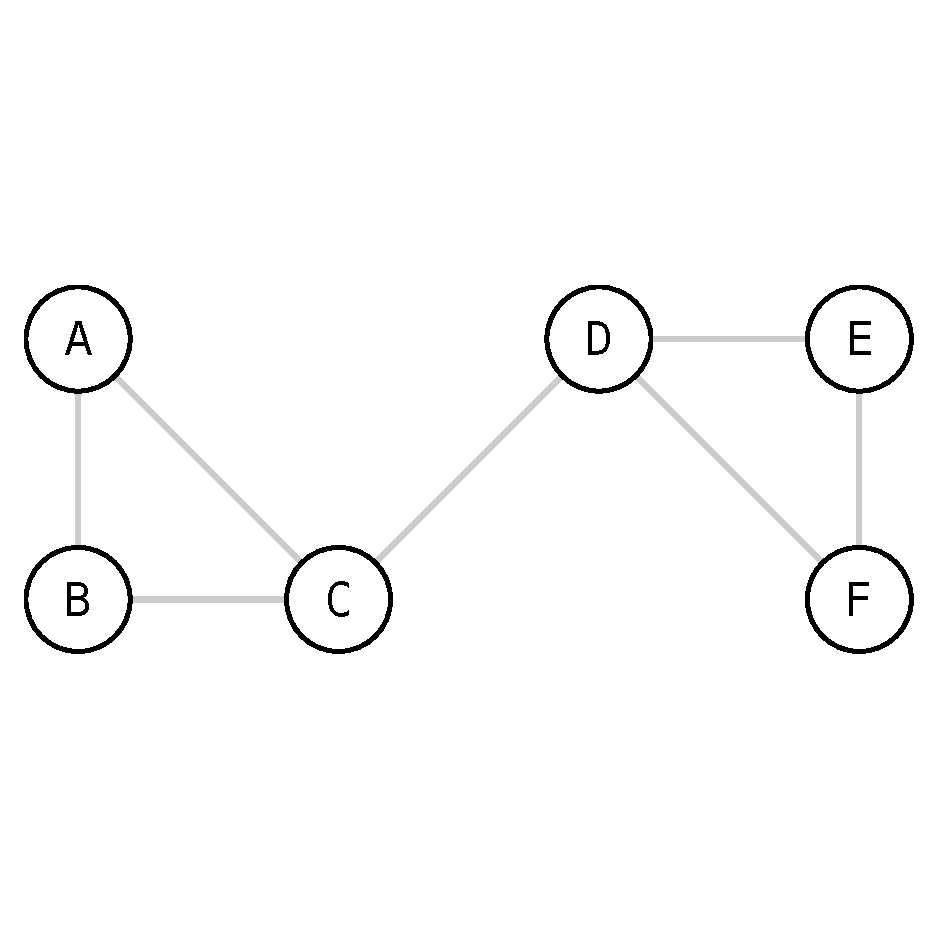
\includegraphics[width=0.46\textwidth]{python/lec04/bridges/bridges-0.pdf}\\[2pt]{\scriptsize Шаг 0. Исходный граф}} &
\shortstack{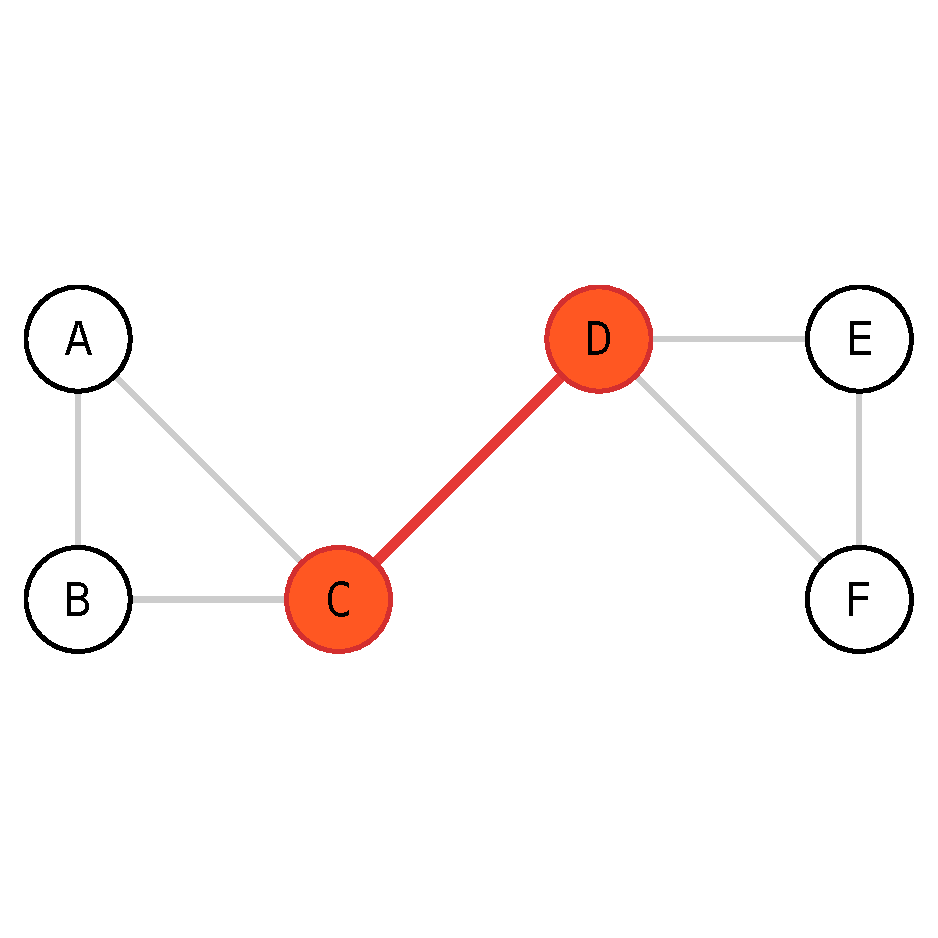
\includegraphics[width=0.46\textwidth]{python/lec04/bridges/bridges-1.pdf}\\[2pt]{\scriptsize Шаг 1. DFS из $A$: ориентируем рёбра по обходу}} \\
\end{tabular}\end{center}
\begin{center}\begin{tabular}{cc}
\shortstack{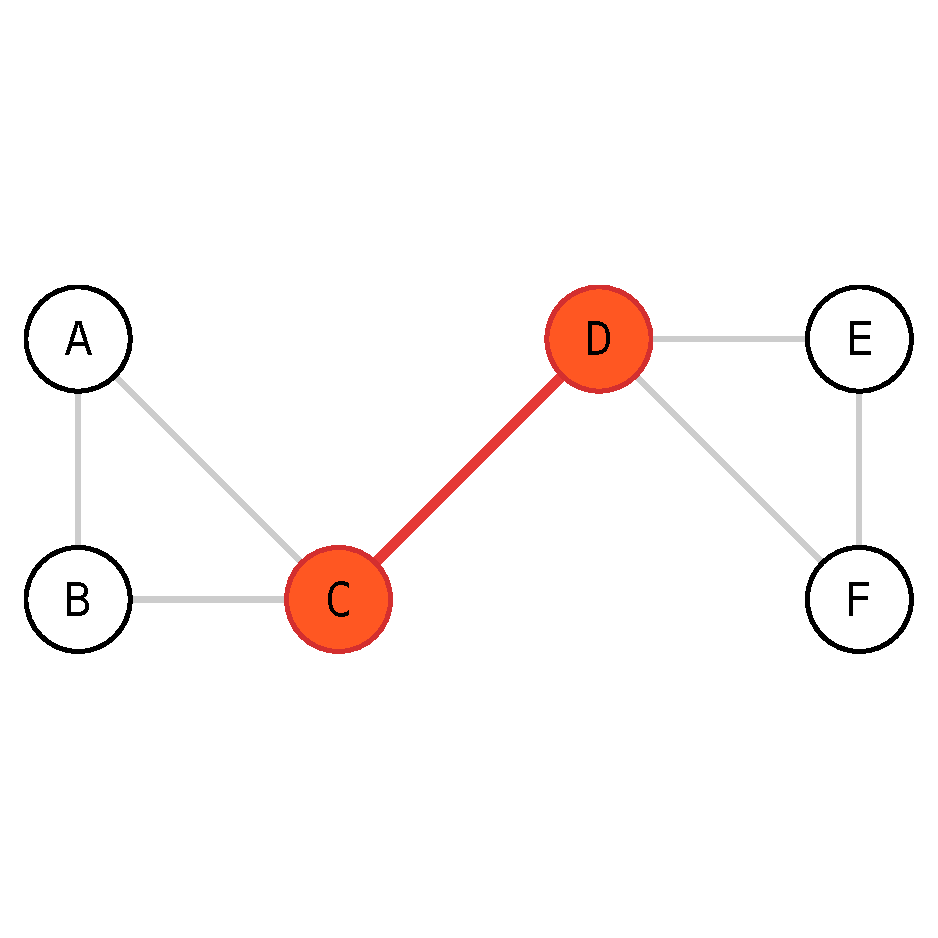
\includegraphics[width=0.46\textwidth]{python/lec04/bridges/bridges-2.pdf}\\[2pt]{\scriptsize Шаг 2. Инвертируем все рёбра}} &
\shortstack{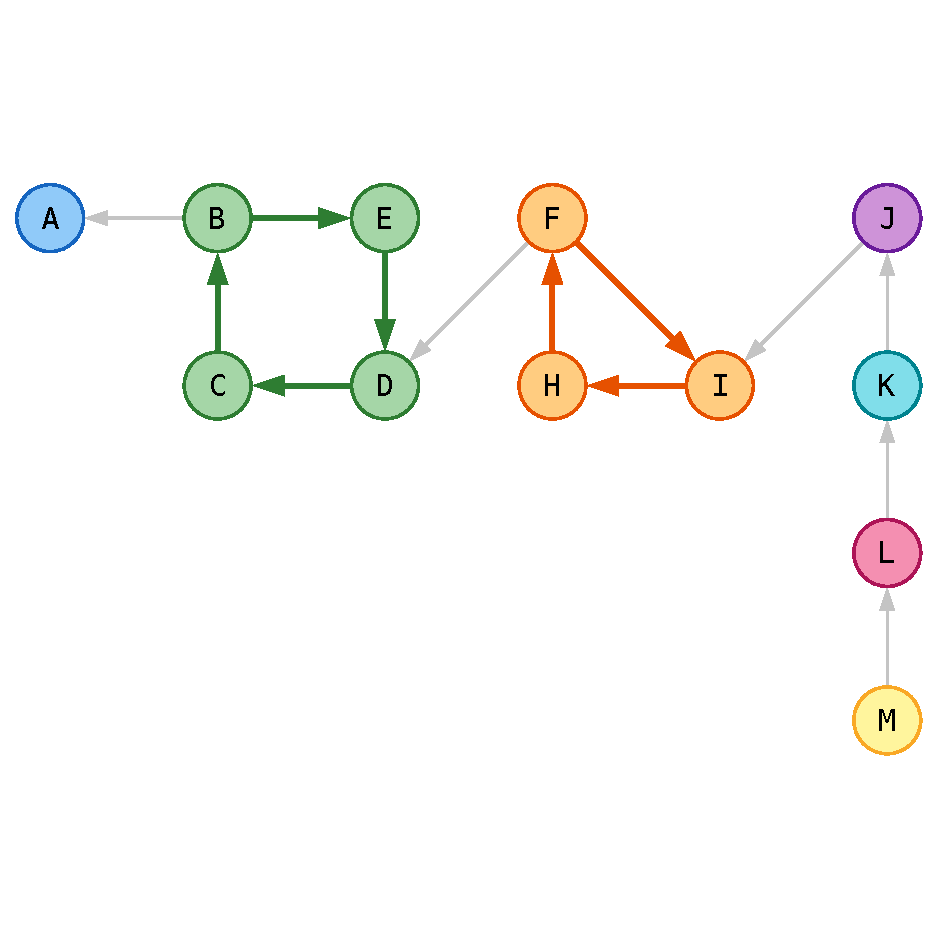
\includegraphics[width=0.46\textwidth]{python/lec04/bridges/bridges-3.pdf}\\[2pt]{\scriptsize Шаг 3. Серия DFS: компоненты --- цветами}} \\
\end{tabular}\end{center}
\begin{center}
\shortstack{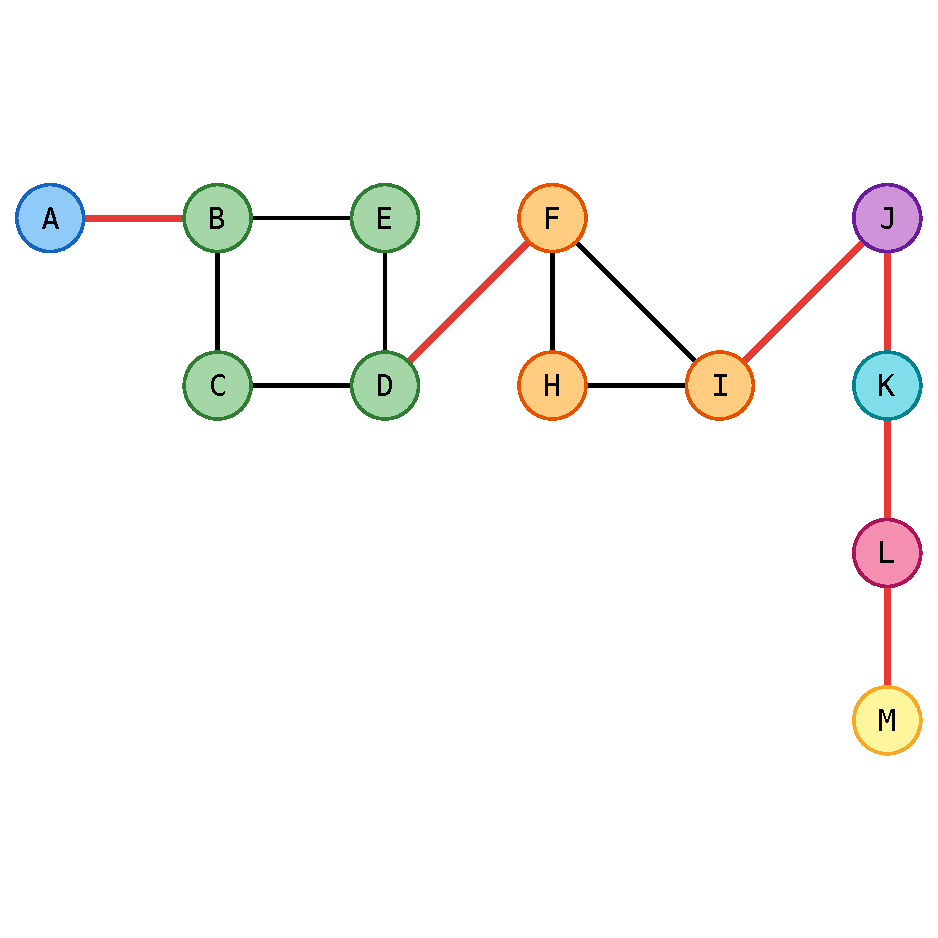
\includegraphics[width=0.5\textwidth]{python/lec04/bridges/bridges-4.pdf}\\[2pt]{\scriptsize Шаг 4. Мосты --- рёбра между разными цветами (красные)}}
\end{center}

\noindent\textit{Комментарии к шагам.} На шаге~1 поиск в глубину из $A$
ориентирует рёбра в порядке обхода:
$A{\to}B{\to}C{\to}D{\to}E$, ребро $E$--$B$ впервые посещается из $E$
(ориентируем $E \to B$); далее $D{\to}F{\to}H{\to}I{\to}J{\to}K{\to}L{\to}M$
и ребро $I \to F$. На шаге~3 серия DFS на инвертированном графе
(в порядке списка $A, B, C, \dots$) даёт компоненты
$\{A\}$, $\{B, C, D, E\}$, $\{F, H, I\}$, $\{J\}$, $\{K\}$, $\{L\}$,
$\{M\}$: из $A$ по инвертированным рёбрам никуда не попасть; из $B$
обходится цикл $B{\to}E{\to}D{\to}C{\to}B$; из $F$ --- цикл
$F{\to}I{\to}H{\to}F$; вершины $J, K, L, M$ остаются поодиночке.

\medskip
\textbf{Мосты данного графа} (рёбра между разными компонентами):
$A$--$B$,\; $D$--$F$,\; $I$--$J$,\; $J$--$K$,\; $K$--$L$,\; $L$--$M$.
\end{algo}
